%Project Narrative
\documentclass[11pt]{article}
\usepackage[margin=1in]{geometry}
\usepackage{color}
\usepackage{graphicx}
\usepackage{url}
\usepackage{multicol}
\usepackage{wrapfig}
\usepackage{amsmath}
\usepackage{amssymb}
\usepackage{caption}
\usepackage{subcaption}
\usepackage[round]{natbib}
\bibpunct[; ]{[}{]}{,}{n}{}{;} 
\bibliographystyle{abbrvnat}
\setcitestyle{authoryear,open={(},close={)}}
\usepackage[usenames,dvipsnames,svgnames,table]{xcolor}
\usepackage[innercaption]{sidecap} % side captions
\sidecaptionvpos{figure}{c}

\begin{document}

\title{\vspace{-5ex}Research Approach: Evolutionary genomics of maize\vspace{-4ex}}
\author{}
\date{}
\maketitle


%Research Approach - not to exceed 1,500 words - of your ongoing and planned research program.
%May include a list of essential references and up to one page of figures.
%Figures and accompanying short legends may be interleaved with the body of the research approach text.
%Figures, legends, and essential references are not included in the 1,500 word limit.


\noindent My research program applies population genetic approaches to understand the genomic basis of evolution change in maize (\emph{Zea mays} ssp. {mays}) and its wild relatives the teosintes.  
Agricultural plants provide a particularly excellent system for basic discovery, with their rich history of basic genetic research, ample modern genetic resources, and the opportunity to sample or replicate genotypes across a wide array of environments.
Among crop plants, maize provides perhaps the best opportunities for basic research and discovery.
In addition to its status as the country's most economically valuable crop, maize is also one of the oldest model organisms, and its rich phenotypic and genetic diversity have enabled a number of basic scientific discoveries, from hybrid vigor \citep{shull1908composition} to the relationship between crossing over and recombination \citep{creighton1931correlation}, meiotic drive \citep{rhoades1942preferential}, and transposable elements \citep{mcclintock1950origin}. 
Maize continues to be an important model in the genomics era \citep{nannas2015genetic}, and the publicly available genomic and phenotypic resources available are unparalleled among other crops: more than 1,000 genomes have been resequenced, more than 20,000 individuals genotyped at $\approx 1$ million SNPs, and association mapping studies now approach scales rarely seen outside of biomedical studies \citep[e.g. 65,000 plots in][]{peiffer2014genetic}.\\

\noindent Maize is particularly well-suited as a model to study plant evolution.
Both domestication and modern breeding can be seen as long-term experimental evolution, and both population genomic \citep{hufford2012comparative} and archaeological \citep{purugganan2011archaeological} data suggest that these are likely relevant and representative of patterns of evolution in natural populations.
Maize has a large genome compared to many other model plants --- the maize reference is 2.3Gb \citep{schnable2009the-b73-maize} ---  but is in fact  close to the median (and below the mean) genome size for most flowering plants \citep{leitch2013genome}, and any understanding of plant evolution would be incomplete without consdiering the structural variation and repeat evolution inherent in such complex genomes.
Finally, the wild relatives of maize, collectively referred to as teosinte, inhabiting a diverse array of environments, and include both endangered species and taxa with large, stable, randomly-mating populations \citep{hufford2012teosinte}.
Because all of these species are closely related, genetic resources developed in maize are often transferred seemlessly to these wild taxa as well \citep[e.g.][]{pyhajarvi2013complex,fang2012megabase}.
Though much effort has been made to apply the genomic resources of maize to accelerate plant breeding, there are surprisingly few efforts to take advantage of maize as a model to more broadly understand plant adaptation and evolution.  
Below I describe current and planned population genetic work in my lab which aims to use maize and teosinte as a model to understand plant adaptation and genome evolution.  

\section*{Domestication}

Plant domestication represents an opportunity to understand not only the genetic basis of evolutionary change, but also how the complex interplay of demography and selection shape modern genetic and phenotypic diversity.
My group has worked to understand the process of selection during domestication, documenting its polygenic nature \citep{hufford2012comparative} and the importance of selection on multiple beneficial mutations \citep{wills2013many} and standing genetic variation \citep{wills2013many, studer2011identification}. 
Our current work focuses not on finding the targets of selection, but instead on how plant domestication has shaped geenetic and phenotypic diversity.
Maize underwent a demographic bottleneck during domestication, reducing its effective population size and thus the efficacy of purifying selection to remove deleterious variants (Figure \ref{fig:purify}A).
Following its domestication, however, maize spread rapidly across the Americas, and this explosive population growth --- our estimates of the current effective size of open-pollinated maize exceed $10^12$ --- has lead to a higher efficacy of selection on new mutations, and patterns of diversity near genes suggest that new mutations in maize are more strongly selected than those in its wild-ancestor (Figure \ref{fig:purify}B).
Population demography also has the potential to change the size, number, and dominance of loci underlying phenotypic traits \citep{lohmueller2014impact,gazave2013population}.
Our future work will utilize data from large-scale association mapping studies in both domesticated and wild populations, coupled with population genetic inference of demographic change and the fitness consequences of new mutations, to study how the process of domestication may have shaped the genetic architecture of phenotypic traits.
Results from these studies will help us better understand the functional consequences of new mutations as well as improve our utilization of genetic diversity to predict phenotype.

\begin{figure*}[tb]
\centering
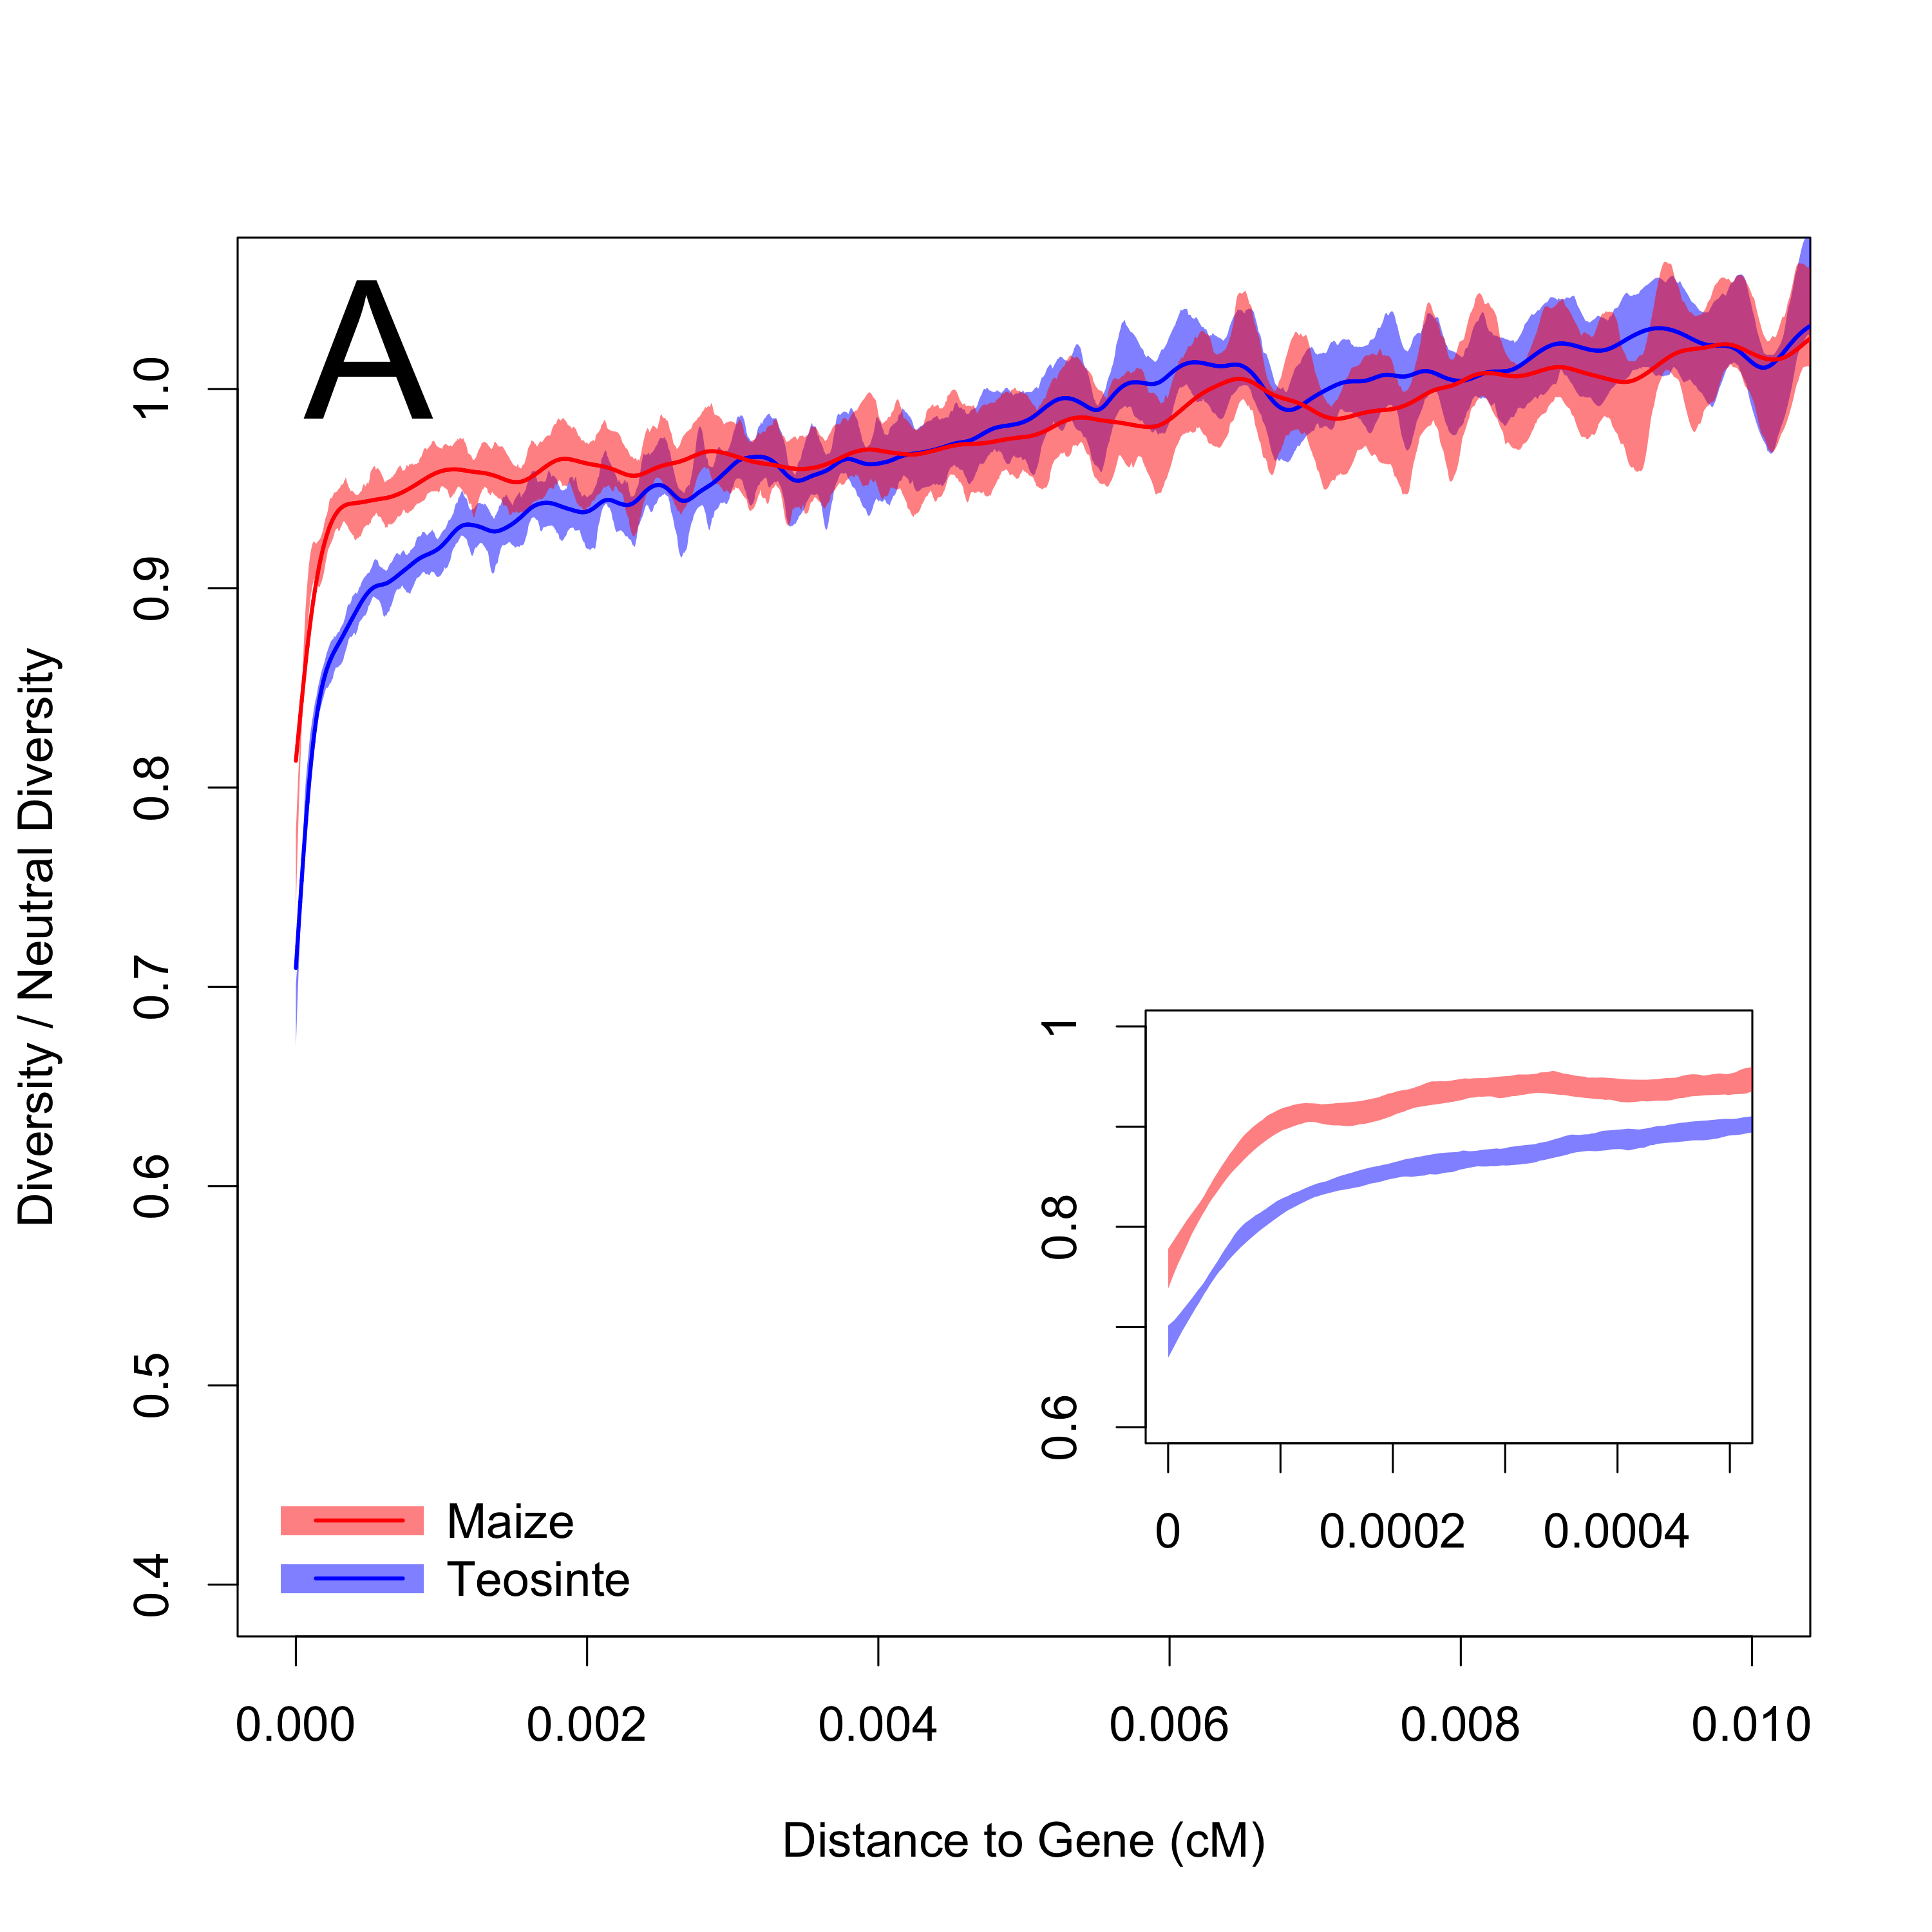
\includegraphics[width=.5\textwidth]{figs/distanceToGene_WithSignificance_Folded2_manuscript.png} 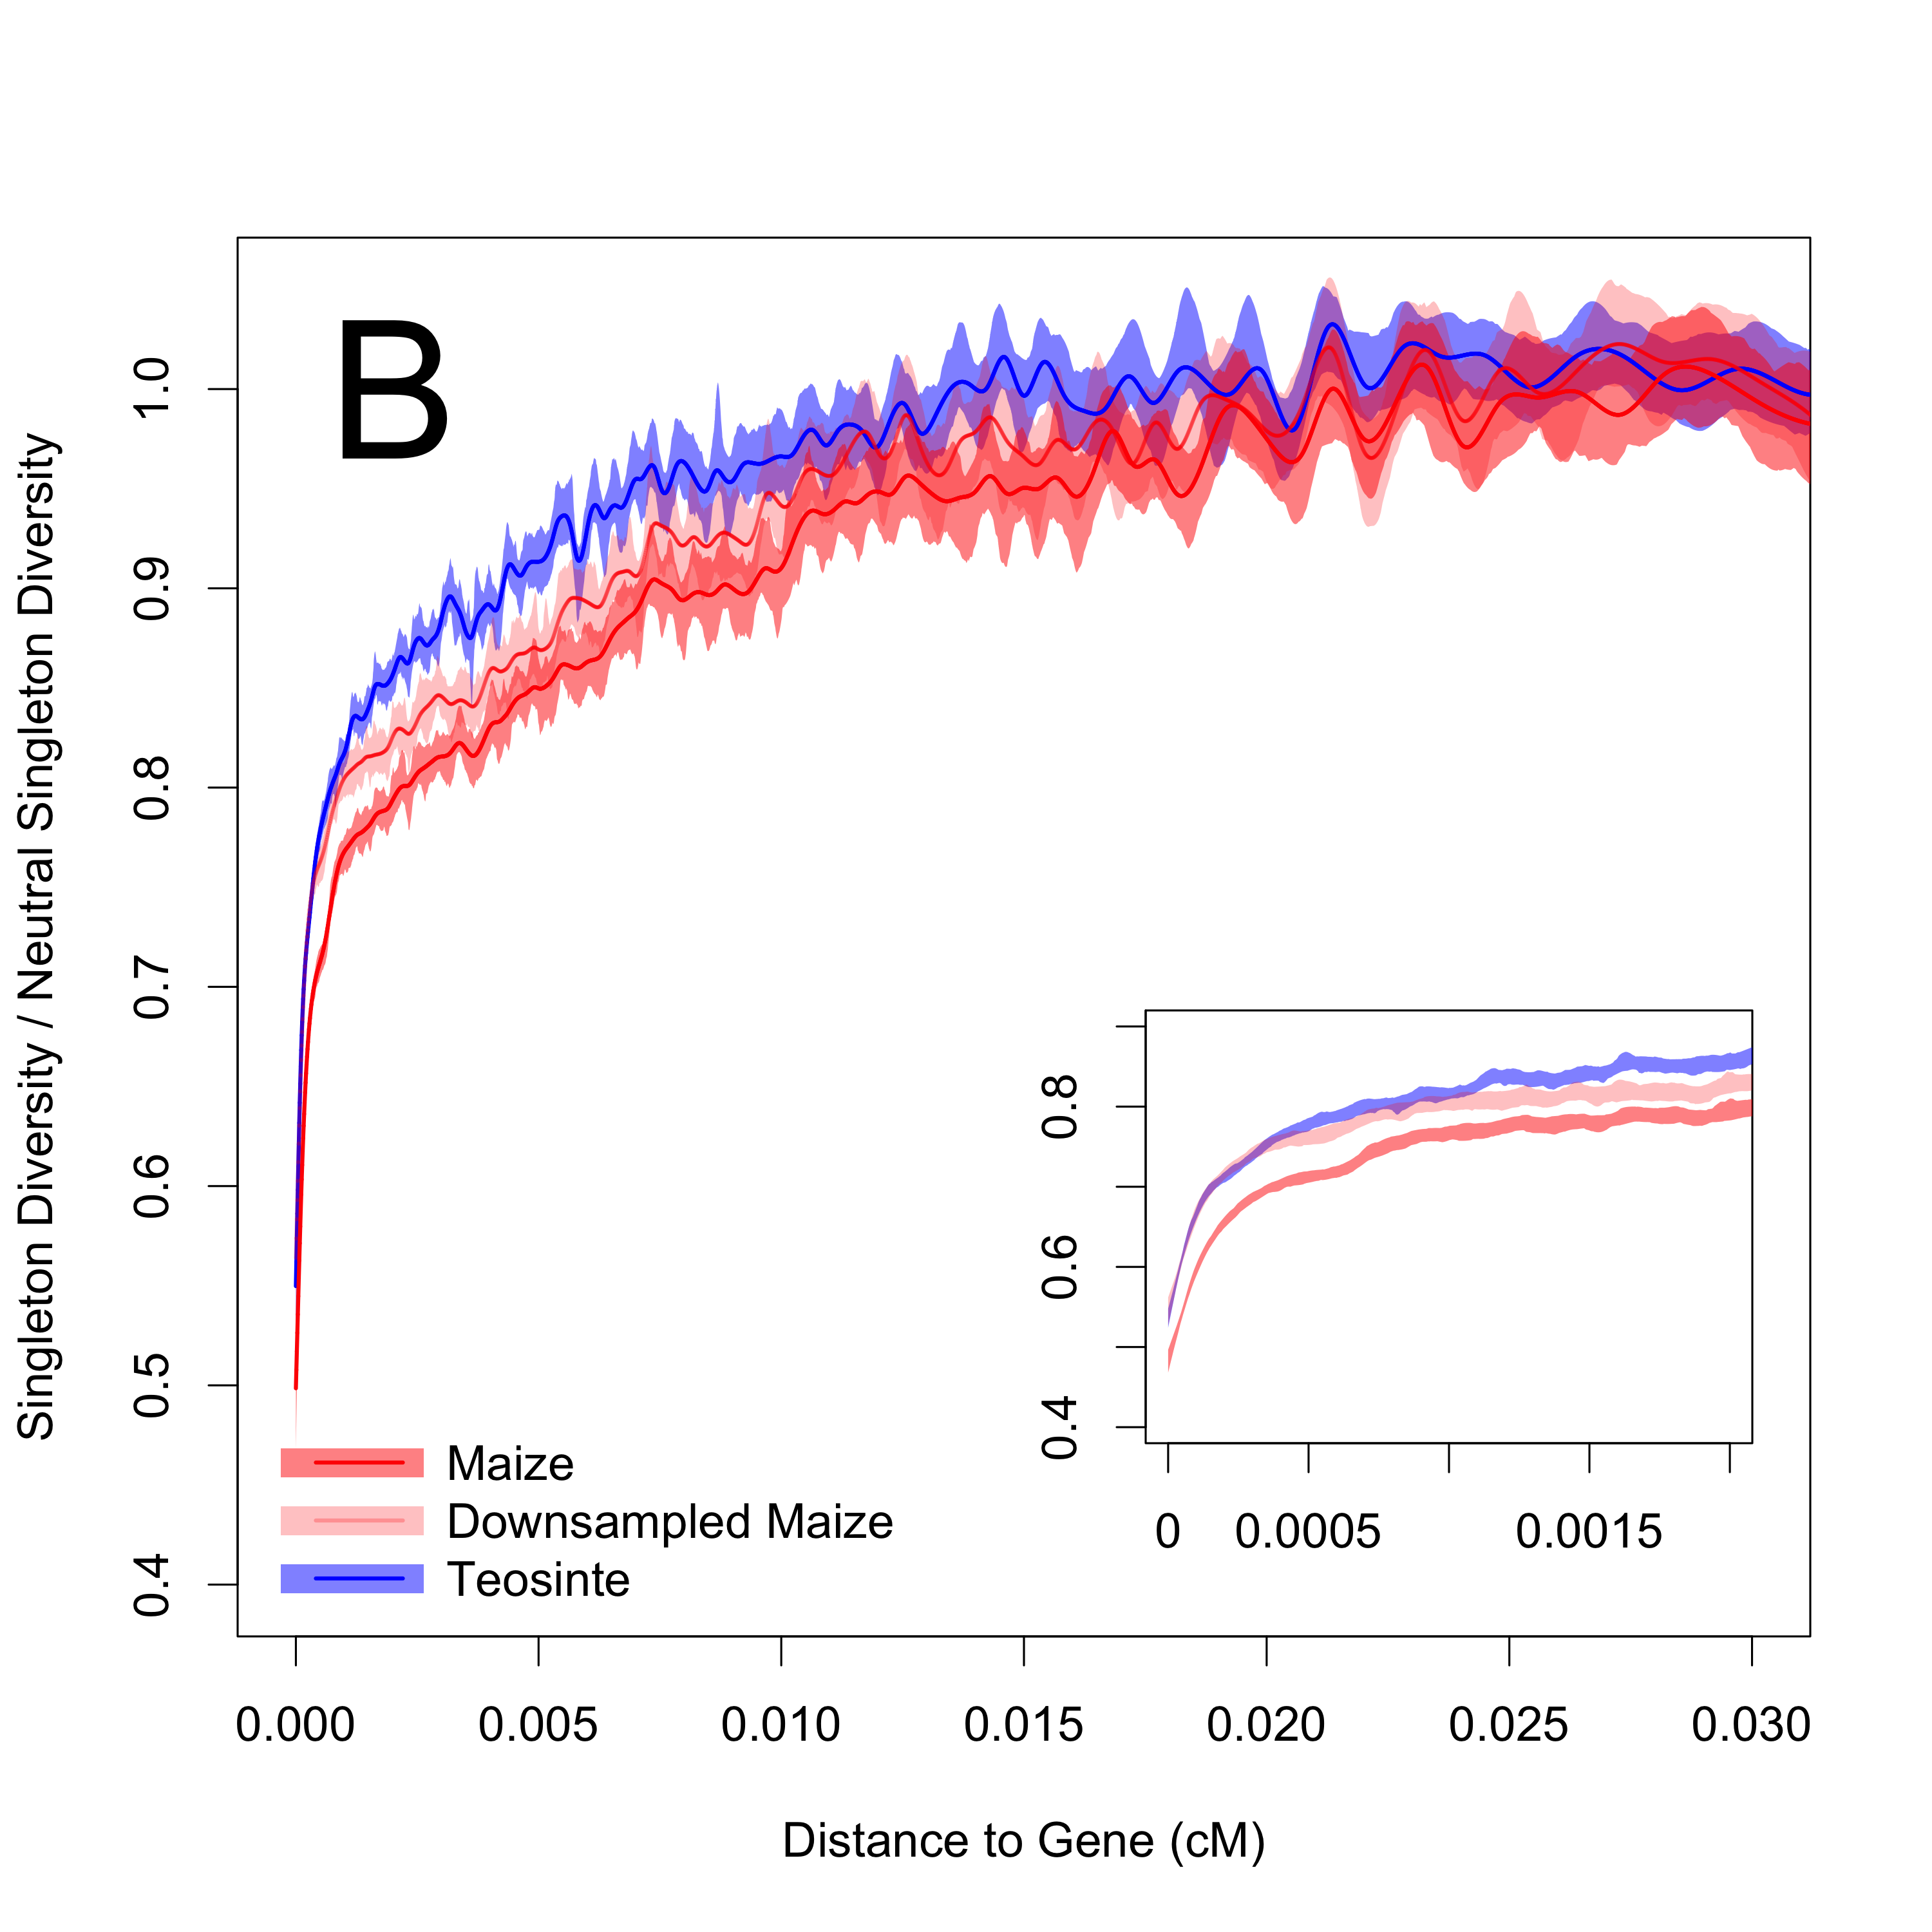
\includegraphics[width=.5\textwidth]{figs/distanceToGene_WithSignificance_Singletons_Downsampled_threeLines_manuscript.png}
\caption{Relative diversity as a function of distance to nearest gene. 
\textbf{A} Pairwise nucleotide diversity $\pi$ is most influenced by intermediate frequency alleles and reflective of long-term demography. 
The stronger effect of purifying selection on $\pi$  in teosinte is consistent with its larger long-term effective population size. 
 \textbf{B} For very recent variants such as those found in a single individuals, purifying selection appears stronger in maize, reflecting its exponential growth following domestication. \label{fig:purify}}
\end{figure*}

{
\color{red}  
\noindent\makebox[\linewidth]{\rule{\linewidth}{0.4pt}}
STOP HERE \\
\noindent\makebox[\linewidth]{\rule{\linewidth}{0.4pt}}
}






\section*{Local adaptation}
% architecture, biotic interactions, climate, introgression

convergent evolution
crop gene flow
inversions regulatory

Protein-coding genes have often been considered the major source of functional variation, and evidence from small model plant genomes such as \emph{Arabidopsis} \citep[e.g.][]{hancock2011adaptation} supports such claims. 
However, most flowering plants have large genomes, like maize, and our work has indicated that in such large genomes other forms of variation likely play a much more important role.  
We have shown that selection has taken extensive advantage of regulatory \citep{swanson2012reshaping,pyhajarvi2013complex} and structural variation --- including inversions \citep{pyhajarvi2013complex,fang2012megabase}, transposable element insertions \citep{studer2011identification,makarevitch2015transposable}, and likely copy-number variation \citep{chia2012maize} --- in both natural and domesticated populations. We believe such noncoding variation will be shown responsible for a substantial fraction of adaptive variation in most plant genomes.
Differences in large complex genomes -- Fraser \citep{fraser2013gene} vs. \citep{pyhajarvi2013complex} or \citep{hancock2011adaptation} and gene expression \citep{hufford2012comparative}



\section*{Experimental evolution}

heterosis.
artificial selection

\begin{figure*}[tb]   
  \begin{center}
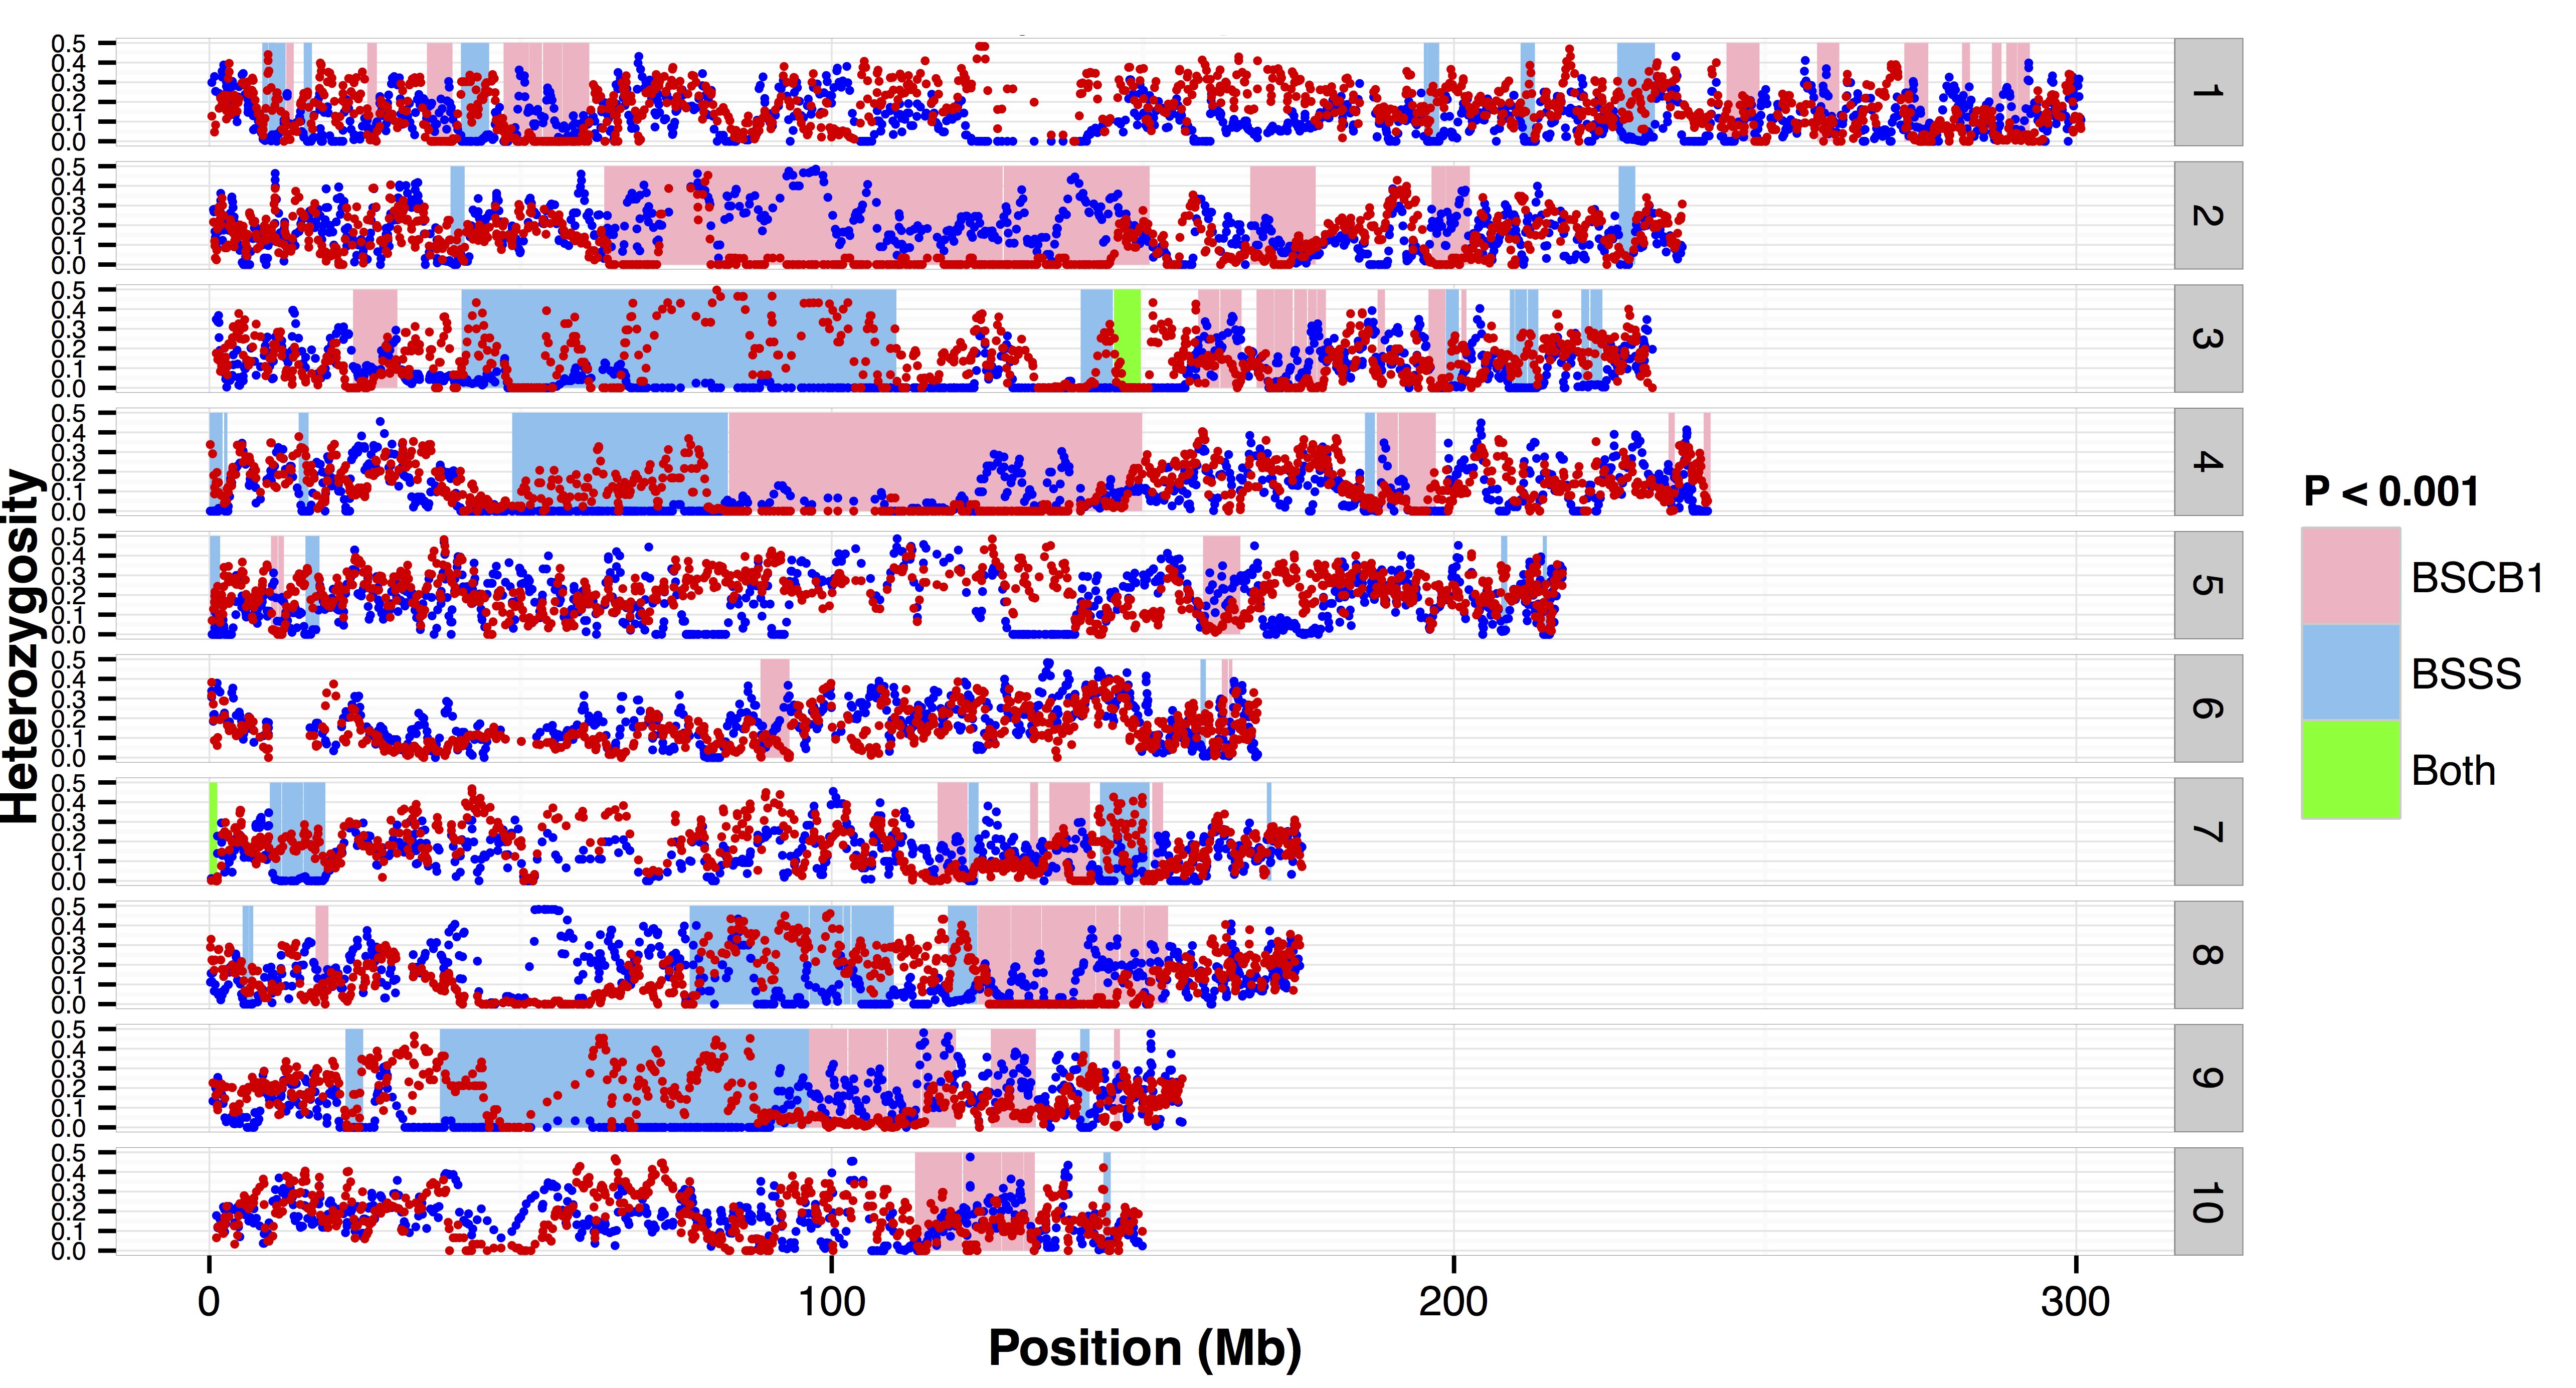
\includegraphics[width=0.8\linewidth]{figs/gerke.png}
   \caption{Heterozygosity across all 10 chromosomes of maize from cycle 16 of the Iowa Reciprocal Recurrent Selection experiment. Heterozygosity values in the BSSS  (blue dots) and BSCB1 (red dots) populations are superimposed in one panel. 2cM windows of heterozygosity lower than 10 of 10,000 simulations ($P<0.001$) are shaded in light blue (BSSS) or pink (BSCB1). Two regions genome-wide show significantly low heterozygosity in both populations and are shaded green.} 
    \label{fig:heterotic}
  \end{center}
\end{figure*}

\section*{Genome evolution}

inversion polymorphisms. likely more common because no underdominance \citep{maguire1966relationship}
TE insertions \citep{studer2011identification, makarevitch2015transposable} and regulation. 
genome size too \citep{tenaillon2011genome}. paul.

michelle stats. 344K insertions, 2728 in genes!

TEs, CNVs, genome size evolution

missing data vs. allele frequencies.
TEs






\begin{figure*}[tb]
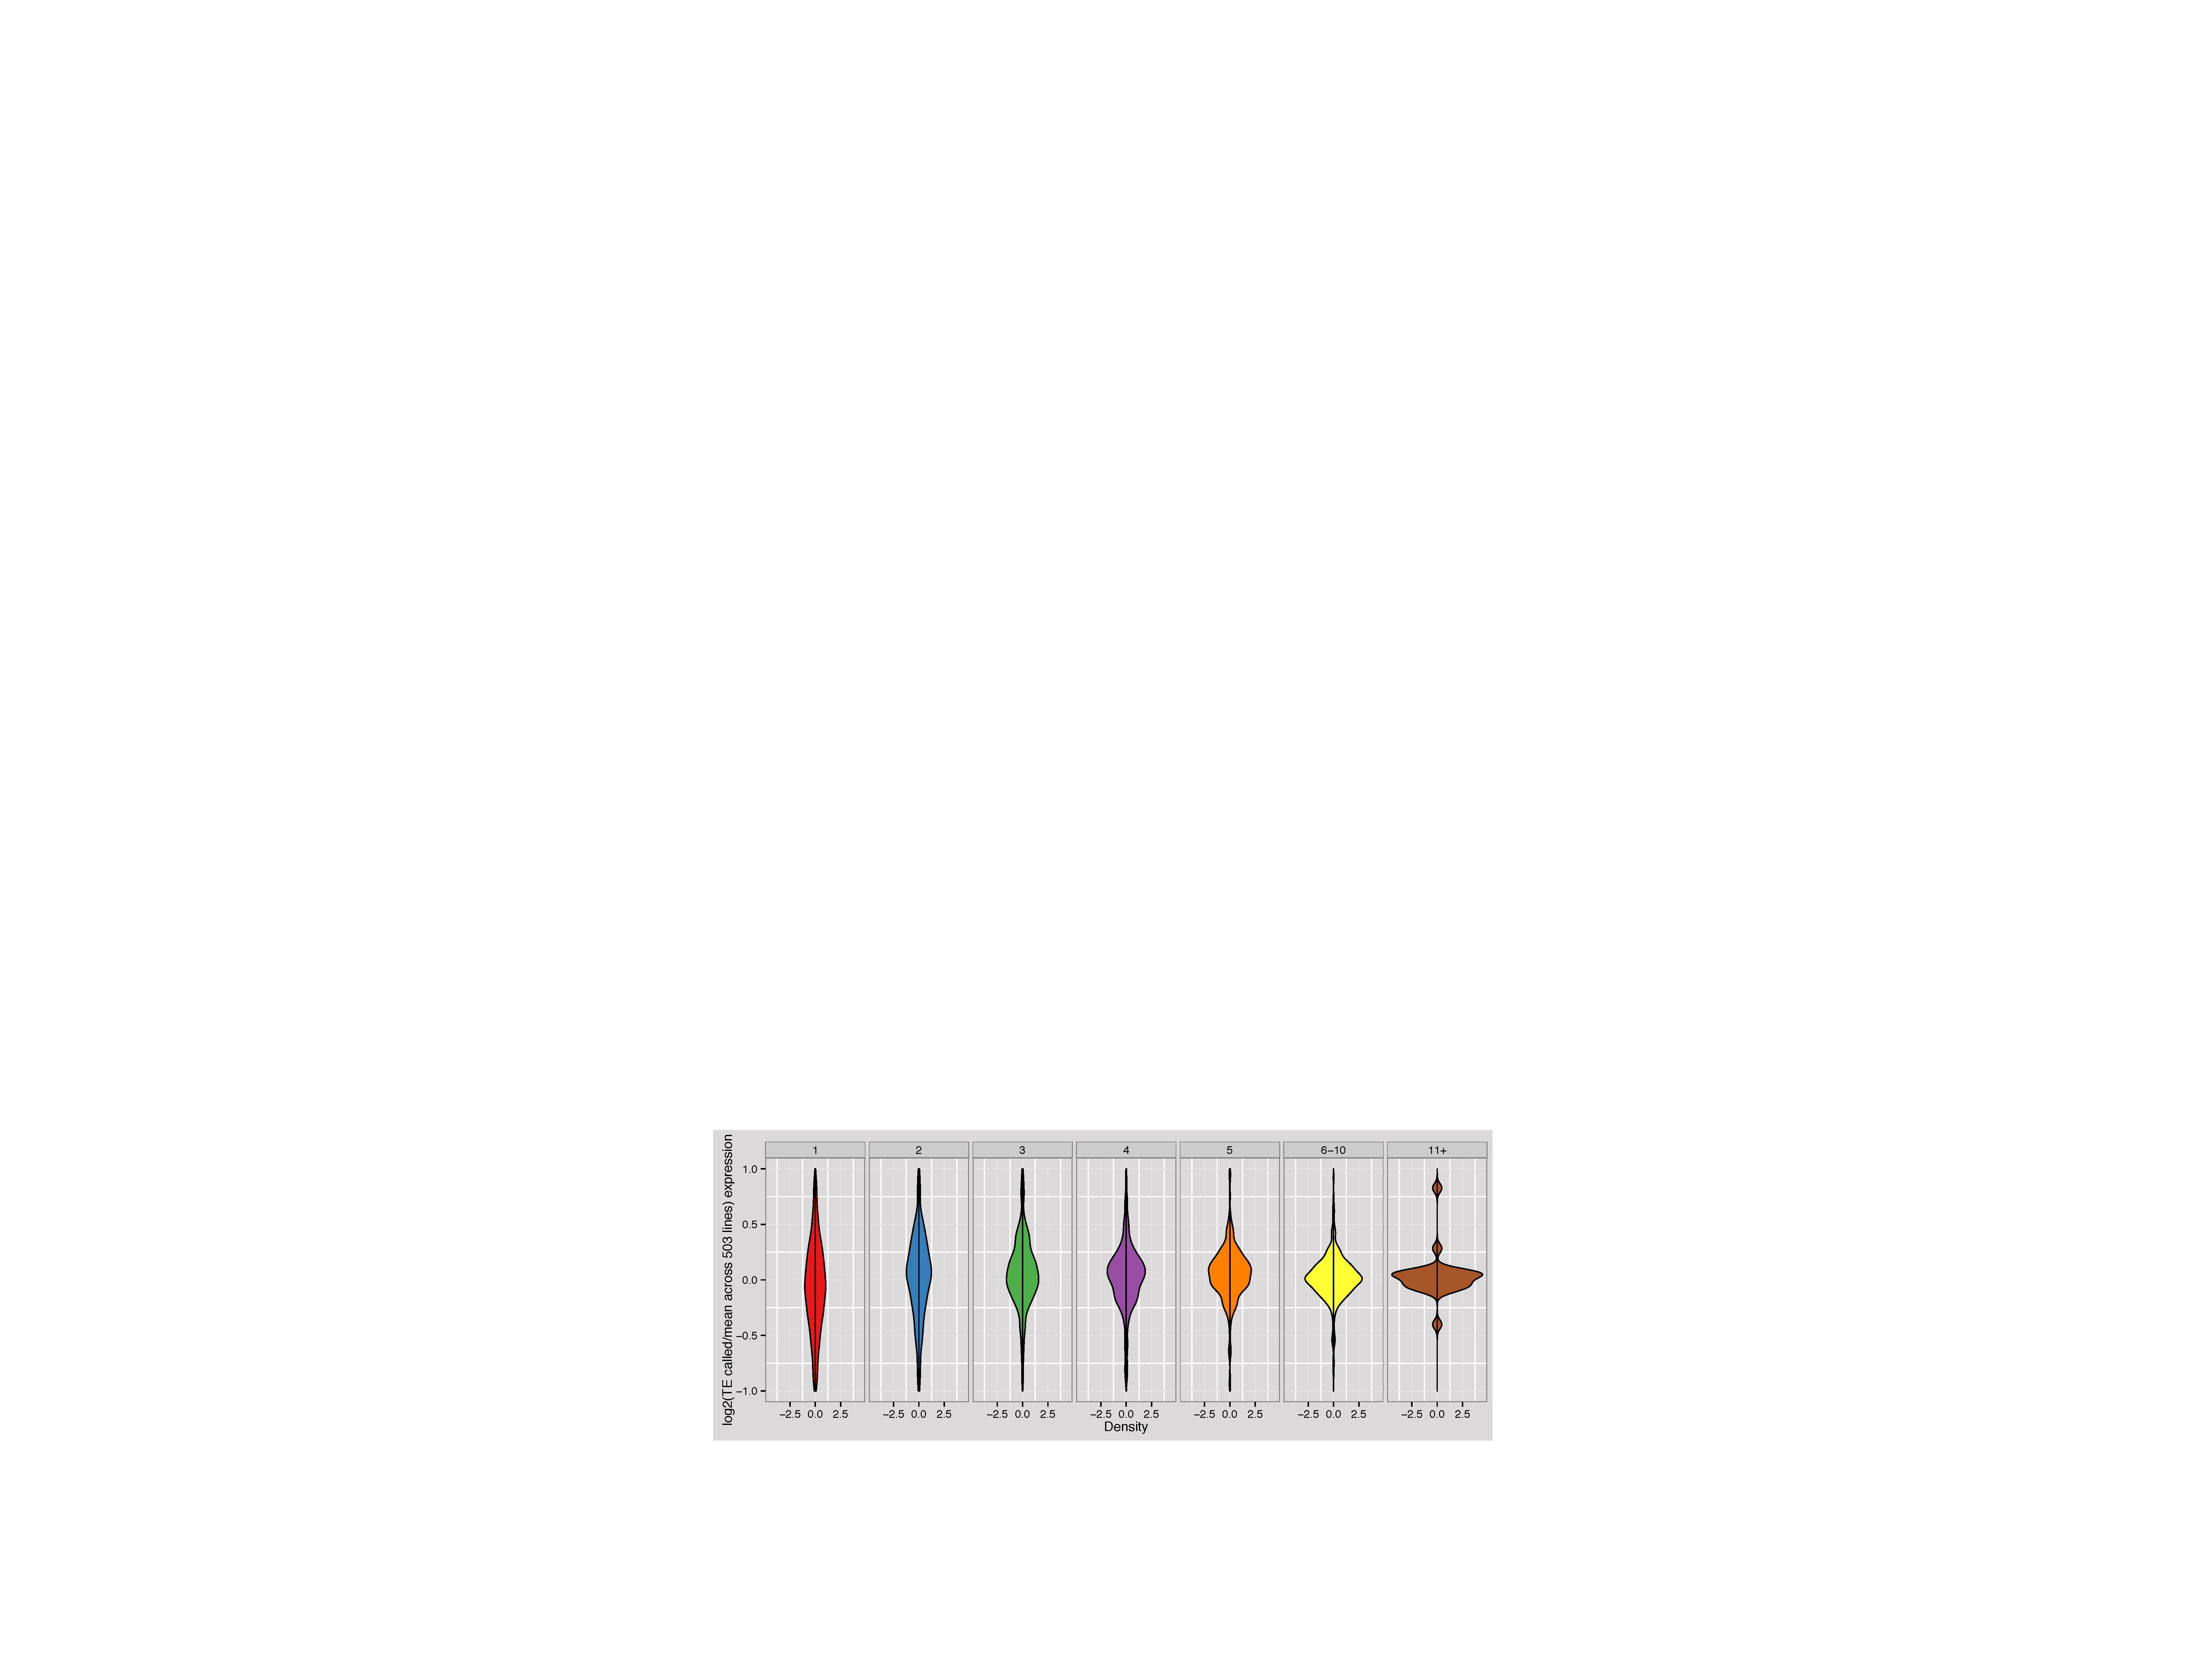
\includegraphics[width=0.45\linewidth]{figs/te_expression.pdf}
\caption{The effect of \emph{de novo} non-reference transposable element insertion on gene expression. Panels show the impact of insertions identified in 1 (far left) to $>10$ (far right) inbred lines in a panel of 23 maize inbreds.  Shown in each panel is the relative expression of genes in inbred lines with the insertion within the annotated gene region to the mean expression of that gene across 500 maize lines \citep{hirsch2014insights}. Recent, low frequency insertions tend to decrease gene expression compared to older, high-frequency insertions.  } 
\label{fig:te_expression}
\end{figure*}

\begin{SCfigure}
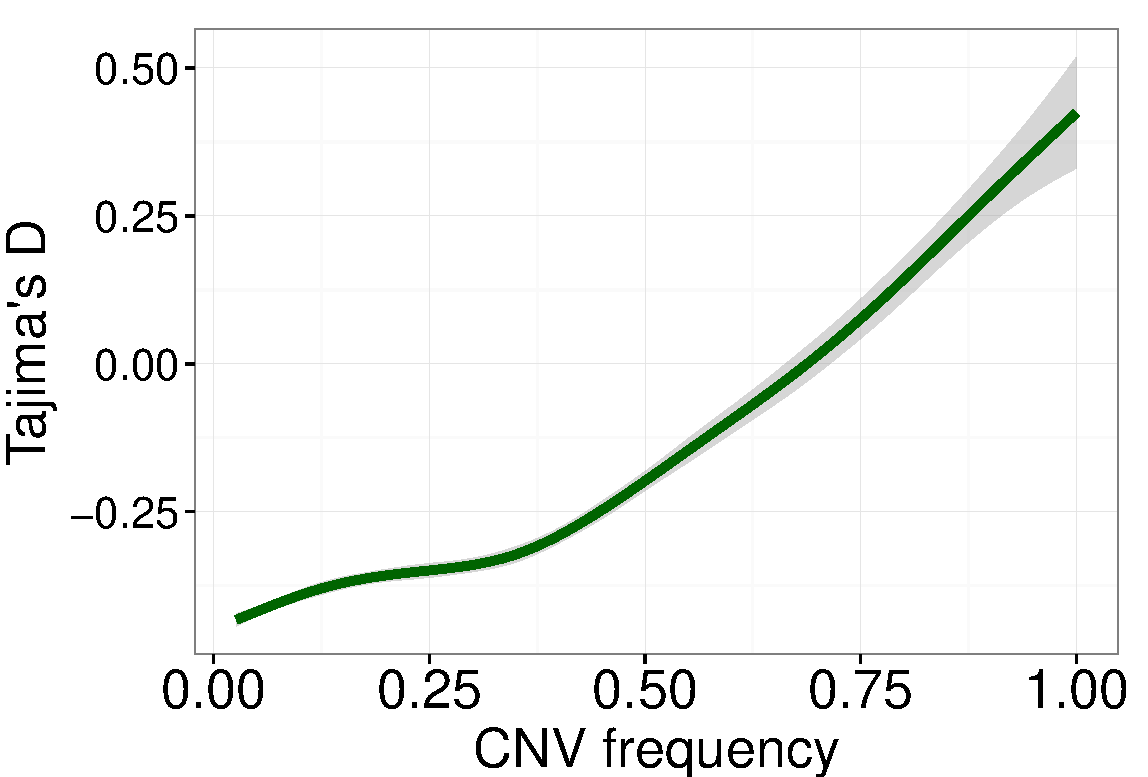
\includegraphics[width=0.3\linewidth]{figs/td_cnv.pdf}
\caption{The effect of copy number variation (CNV) on estimates of Tajima's D, a measure of the allele freqeuncy spectrum. In regions with no CNV, Tajima's D is negative consistent with population expansion. Tajima's D is inferred to be strongly postiive in regions with high-frequency CNVs, however, which could be (erroneously) interpreted as population decline or balancing selection.} 
\label{fig:tajd}
\end{SCfigure}
%

%\section*{Notes}
%
%\citep{peischl2015expansion} predict more u-shaped SFS in expanded pops, also more homozygous deleterious. this is seen in humans. Li's results in maize
%
%\citep{fu2014characteristics}
%``Indeed, a substantial amount of the higher density of deleterious alleles in EA individuals in the simulated data is attributable to weakly deleterious mutations $(|s| \approx 10^{-4})$''
%
%\citep{balick2013response} show weighted sum of the SFS can be used to differentiate recessive vs. not at deeteirous sites.
%
%\citep{lohmueller2014impact} 
%``Under a model where a mutation's effect on a trait is correlated with its effect on fitness, rare variants explain a greater portion of the additive genetic variance of the trait in a population that has recently expanded than in a population that did not recently expand. Further, when using a single-marker test, for a given false-positive rate and sample size, recent population growth decreases the expected number of significant associations with the trait relative to the number detected in a population that did not expand. However, in a model where there is no correlation between a mutation's effect on fitness and the effect on the trait, common variants account for much of the additive genetic variance, regardless of demography.''
%
%\citep{tennessen2012evolution} Shows vast majority of functionally important alleles rare, attributes to explosive population growth and weak purifying selection
%
%\citep{hufford2013genomic} \citep{hufford2012comparative}




\newpage
\bibliography{jri.bib}
\end{document}
